\documentclass[conference]{IEEEtran}
\IEEEoverridecommandlockouts
% The preceding line is only needed to identify funding in the first footnote. If that is unneeded, please comment it out.

\usepackage[bahasa]{babel}

\usepackage[noadjust]{cite}
\usepackage{amsmath,amssymb,amsfonts}
\usepackage{algorithmic}
\usepackage{graphicx}
\usepackage{textcomp}
\usepackage[table]{xcolor}

\def\BibTeX{{\rm B\kern-.05em{\sc i\kern-.025em b}\kern-.08em
    T\kern-.1667em\lower.7ex\hbox{E}\kern-.125emX}}
\begin{document}

\title{Peningkatan Kinerja Modul Pencocokan Pola dalam Sistem Deteksi Intrusi Snort Menggunakan GPU\\
{\footnotesize \textsuperscript{*}Note: Sub-titles are not captured in Xplore and
should not be used}
\thanks{Identify applicable funding agency here. If none, delete this.}
}

\author{
\IEEEauthorblockN{Afrizal Fikri}
\IEEEauthorblockA{{School of Electrical Engineering and Informatics} \\
{Institut Teknologi Bandung}\\
{Bandung, Indonesia} \\
afrizalf96@gmail.com}
\and
\IEEEauthorblockN{Achmad Imam Kistijantoro}
\IEEEauthorblockA{{School of Electrical Engineering and Informatics} \\
{Institut Teknologi Bandung}\\
{Bandung, Indonesia} \\
imam@informatika.org}
}

\maketitle

\begin{abstract}
    Kemajuan teknologi telah memberikan kontribusi pada pertumbuhan pesat penggunaan data digital. Di era digital ini, banyak data fisik telah diubah menjadi digital. Di antara mereka, banyak data rahasia juga terjadi. Dengan demikian, jaminan keamanan menjadi penting juga. Salah satu titik masuk dari penggunaan berbahaya tersebut berasal dari sisi server. Memastikan otoritas pada server yang menggunakan sistem deteksi intrusi jaringan (NIDS) dapat mengambil sumber daya dan waktu yang sangat besar. Salah satu bagian penting dari NIDS adalah string yang cocok dengan bagian di dalam alat analisa. Berdasarkan alasan ini, makalah ini bertujuan untuk meningkatkan kecepatan deteksi yang cocok untuk memaksimalkan keseluruhan sistem throughput menggunakan GPU bukan CPU. Berdasarkan percobaan dan pengujian, solusi yang diusulkan memiliki waktu operasi yang jauh lebih baik dibandingkan dengan solusi linear state of the art dengan tetap menjaga akurasi.
\end{abstract}

\begin{IEEEkeywords}
    pattern matching; intrusion detection; GPU; parallel computation; CUDA
\end{IEEEkeywords}

\section{Introduction}
% The advancement of technology has given contributions to the rapid growth of the use of digital data. In this digital era, lots of physical data have been transformed into the digital ones. One example of the use of digital data is the digital biometric fingerprint data on the Electronic Identity Card (KTP-el). 

% To identify a person, fingerprint matching can be used. There are some techniques to do fingerprint matching. One of popular technique is minutia-based fingerprint matching [1]. The technique can be classified into two categories, nearest neighbor-based and fixed radius-based. Each category has their own advantages and disadvantages. However, there is a technique that combines their advantages without having their drawbacks, i.e. Minutia Cylinder-Code (MCC). 

% Fingerprint matching is a problem, especially in a country that has a large population. According to Indonesian 2010 census, it was found that the total population of Indonesia was approximately 237.641.326 at that time [2]. In regard to this matter, the process of analyzing their fingerprints data could take extremely long time if it done linearly, which is what is currently happening. Thus, there is a need for a parallel fingerprint matching.

Salah satu sumber daya yang penting untuk dilindungi yaitu \emph{server}. Banyak aspek security yang terdapat pada \emph{server} dan dapat dengan mudah diserang \cite{owasp}. Solusi untuk pengamanan \emph{server} dari \emph{request} berbahaya adalah dengan menggunakan sistem deteksi intrusi jaringan atau \emph{network intrusion detection system} (NIDS). NIDS berfungsi mengenali kemungkinan serangan dari \emph{request} yang diterima pada \emph{server} atau \emph{client} sebagai tindakan pencegahan. Ketika \emph{request} dianggap berbahaya, maka dapat dilakukan tindakan lanjutan untuk mencegah kerusakan lebih lanjut pada aset. NIDS yang melakukan tindakan preventif seperti ini disebut juga NIPS (\emph{network intrusion prevention system}).

Salah satu contoh NIDS yang banyak digunakan adalah NIDS Snort. Snort adalah salah satu NIDS berbasis \emph{signature} yang mencocokan paket dengan \emph{rule} yang telah dikumpulkan. \emph{Rule} Snort terdiri dari beberapa komponen yang bertujuan mengenali \emph{host} asal, \emph{host} tujuan, dan isi paket jaringan. \emph{Rule} yang digunakan berasal dari riset para pakar keamanan dan terus diperbaharui mengikuti pola-pola serangan terbaru.

Karena adanya peningkatan kecepatan \emph{traffic} internet dan banyaknya serangan yang terjadi, maka dibutuhkan NIDS yang mampu melakukan deteksi dengan lebih cepat. Salah satu \emph{bottleneck} dalam pengecekan paket adalah banyaknya \emph{rule} yang harus dicocokkan \cite{pcre2007}. Sehingga, peningkatan secara signifikan dapat dicapai salah satunya dengan meningkatkan kemampuan komputasi untuk pencocokan banyak paket secara paralel. Pemanfaatan \emph{multithreading} pada \emph{multicore processor} telah dikembangkan untuk mempercepat kinerja NIDS \cite{multi2004}.

Selain mengoptimalkan penggunaan CPU, alternatif yang dapat digunakan yaitu penggunaan \emph{general purpose} GPU (GPGPU) \cite{4482891}. Dapat juga menggunakan prosesor yang mudah dikustomisasi seperti ASIC atau FPGA \cite{fpga2008}. GPGPU banyak digunakan karena perangkat yang mudah didapatkan, multiguna, dan hanya membutuhkan lebih sedikit kustomisasi daripada ASIC dan FPGA. Selain itu, perbandingan kinerja antara GPGPU dan ASIC atau FPGA tidak terlalu jauh tanpa melakukan kustomisasi lebih lanjut di tingkat \emph{low level} \cite{gnort2008}. Maka, Tugas Akhir ini akan fokus untuk melakukan eksperimen terhadap metode pencocokan \emph{string} pada NIDS yang berbasis GPGPU.

% Parallel processing can be done with multicore CPU, multicore GPU, or multicomputer. The difference between CPU and GPU is how they process task [3]. CPU only has several cores designed to process sequentially, while GPU has thousands of cores designed to do tasks in parallel.

% Based on previous statements, this paper aims to optimize fingerprint matching using Minutia Cylinder-Code with GPU. The optimization will be evaluated and the performance will be compared to the baseline.

Perkembangan teknologi telah begitu cepat 

\section{String Matching}
Secara umum, ada dua jenis pencocokan string: tunggal pencocokan pola string dan pencocokan pola string. Kami akan fokus ke pencocokan string pola multi. Ada beberapa algoritma terkenal untuk pencocokan string pola multi: Algoritma Aho-Corasick \cite{ahoc1975}, Commentz-Walter \cite{walter1980}, dan Wu-Manber \cite{wu92}. Tulisan ini akan mencoba menerapkan variasi algoritma Aho-Corasick.

    \subsection{Aho-Corasick Algorithm}
    Algoritma Aho-Corasick adalah jenis algoritma pencocokan string yang bekerja dengan mencocokkan tiap string ke kamus. Kamus akan berisi semua pola untuk dicocokkan dalam bentuk \emph{state machine}.
    
    Dalam algoritma ini, operasi pencocokan dilakukan dengan menelusuri \emph{state machine} untuk tiap karakter dalam string input. Jika sampai pada \emph{final state}, maka string input dianggap cocok dengan salah satu pola. Pencocokan berlanjut hingga string input berakhir. 

    \begin{figure}[htbp]
        \centerline{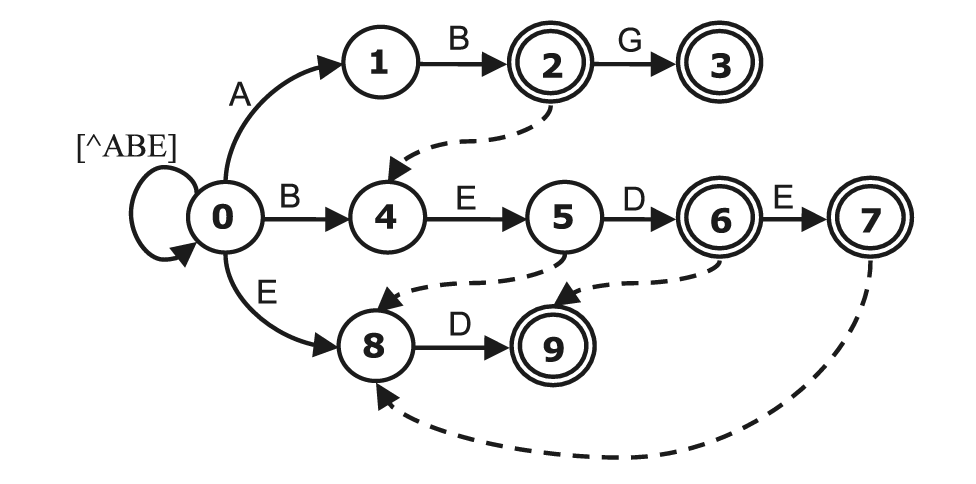
\includegraphics[width=0.4\textwidth]{../src/resources/aho-c.png}}
        \caption{Example state machine of Aho-Corasick dictionary.}
    \end{figure}

    Aho-Corasick menggunakan \emph{failure function} untuk melakukan \emph{backtrack} setelah berhenti di salah satu \emph{final state}. \emph{Failure function} akan menunjuk dari \emph{final state} sekarang ke prefiks pola terpanjang yang cocok dengan sufiks dari pola yang saat ini dicocokkan \cite{ahoc1975}. \emph{Failure function} mengurangi redundansi untuk sekuens yang telah dilewati. Dengan metode ini, semua pola yang ada dalam kalimat dapat dicocokkan dengan sekali penelusuran dan mengurangi kompleksitas dari $O(mn)$ to $O(n)$. 

    Dalam algoritma ini, akses memori menjadi \emph{bottleneck}. Setiap operasi penelusuran akan mengambil satu entri dari tabel. Karena akses memori lebih mahal daripada komputasi, algoritma ini terbatas dengan memori (\emph{memory bound}) \cite{lin2013}.

    \subsection{Data Parallel Aho-Corasick}
    Untuk membuat Aho-Corasick menjadi \emph{multithreading}, beban pencocokan perlu dibagi ke setiap \emph{thread}. Salah satu caranya adalah dengan mempartisi input menjadi beberapa bagian dan kemudian setiap \emph{thread} akan mencocokkan tiap bagian yang berkorespondensi terhadap kamus. Namun, jika ada pola yang menjangkau beberapa bagian sekaligus, pola tidak akan dikenali pada kedua \emph{thread}. Masalah ini dikenal sebagai \emph{boundary matching problem}. Sehingga perlu memperpanjang sesuai dengan panjang pola terpanjang. Akses memori meningkat menjadi $O((n/s + m) * s) = O(n + ms)$ dengan $s$ adalah banyak bagian. 

    \begin{figure}[htbp]
        \centerline{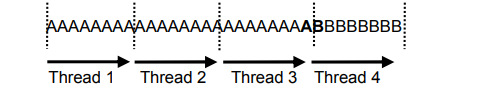
\includegraphics[width=0.4\textwidth]{../src/resources/boundary.png}}
        \caption{Pattern \textbf{AB} not recognized by both thread 3 and 4}
    \end{figure}

    \subsection{Parallel Failureless Aho-Corasick}
    Metode lain untuk mengadaptasi Aho-Corasick dengan \emph{multithreading} adalah membagi \emph{thread} ke semua \emph{byte} karakter. Setiap \emph{thread} akan mencocokkan pola yang dimulai dengan karakter yang berkorespondensi dan selesai ketika ada \emph{final state} atau tidak ada transisi yang valid pada karakter \cite{lin2013}. Konsekuensinya adalah setiap \emph{thread} paling banyak hanya akan cocok dengan satu pola.
    
    Dengan demikian, \emph{failure function} tidak diperlukan lagi. Selain itu, \emph{boundary matching problem} tidak akan terjadi dengan menggunakan pendekatan ini. Pendekatan ini dinamakan juga sebagai \emph{Parallel Failureless Aho-Corasick} (PFAC).

    \begin{figure}[htbp]
        \centerline{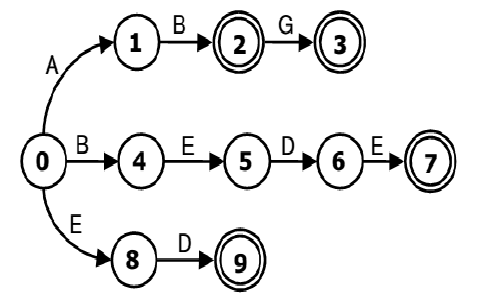
\includegraphics[width=0.4\textwidth]{../src/resources/pfac.png}}
        \caption{State machine without failure function}
    \end{figure} 

\section{Related Works}

    \subsection{Utilization of Double Buffering Scheme, Texture Memory and Pinned Memory}

        Dalam tulisan ini, implementasi pencocokan berbasis GPU telah diusulkan menggunakan algoritma Aho-Corasick. Selain pemanfaatan GPU multithreading, ada beberapa penyesuaian untuk mengimpor Aho-Corasick ke GPGPU. Mesin negara dibangun menggunakan tabel transisi pada tabel 2D pada memori tekstur. Berdasarkan eksperimen, penerapan ini meningkatkan kinerja sebesar 19\% \cite{gnort2008}.
        
        Untuk skema transfer memori, skema \emph{double buffering} diusulkan. Paket akan di-batch dalam satu \emph{buffer}. Setiap kali \emph{buffer} penuh, semua paket ditransfer ke GPU dalam satu operasi. Mentransfer dari perangkat ke host juga dilakukan dengan cara yang sama. Semua hasil akan dikumpulkan di \emph{buffer} kedua dan ditransfer ketika penuh.
        
        Trik optimasi lain yang digunakan adalah menggunakan \emph{pinned memory}. Kedua \emph{buffer} in host akan manggunanakan \emph{pinned memory} untuk mengurangi swappiness. Dan juga \emph{pinned memory} memungkinkan transfer secara langsung tanpa melalui CPU atau \emph{direct memory access} (DMA) dan mengurangi kebutuhan komputasi dan latensi. Desain ini dapat meningkatkan kinerja sistem hingga 3,2 kali lebih tinggi daripada implementasi menggunakan \emph{multithreading} pada CPU.

    \subsection{Scalable Architecture for Maximizing GPU Utilization}

        Dengan profiling, disimpulkan bahwa hambatan terjadi pada 3 komponen: akuisisi paket, pencocokan string pola multi, dan pencocokan aturan opsi oleh ekspresi reguler. Selain itu, di dalam komponen senar string saja, rata-rata utilisasi GPU masih rendah. Makalah ini menerapkan perbaikan arsitektur di sekitar NIDS. \ textcolor {red} {Metode yang diusulkan} adalah pipelining dan payload batching. Pipelining digunakan untuk memisahkan penggunaan benang dalam transfer dan pencocokan. Dan dengan arsitektur ini, NIDS dapat diskalakan ke beberapa GPU dan CPU contoh inti \ cite {kargus2012}.
        
        Perbaikan yang dicapai dengan metode ini adalah sekitar 1,5 hingga 4 kali lebih tinggi dibandingkan dengan garis dasar Snort. Evaluasi dilakukan menggunakan CPU ganda Intel X5680 dengan masing-masing 12 core dan GPU ganda NVIDIA GTX 580. NIDS dijalankan di bawah lalu lintas jaringan dengan kapasitas sekitar 40 Gbps dan bisa mencapai throughput 25,2 Gbps.

    \subsection{Failureless Aho-Corasick by Maximizing Shared Memory Usage}

        Salah satu cara untuk melakukan pencocokan Aho-Corasick adalah dengan menetapkan setiap byte input ke setiap utas secara bersamaan. Kemudian setiap utas akan melakukan pencocokan \ textcolor {red} {begin} dengan byte assined. Pencocokan berhenti setiap kali keadaan akhir atau transisi tidak valid terjadi. Pendekatan ini tidak memerlukan fungsi kegagalan. Sehingga setiap utas hanya bertanggung jawab untuk mencocokkan paling banyak satu pola \ cite {lin2013}.
        
        Pendekatan baru ini memanfaatkan penggabungan memori dalam GPU sehingga byte yang berurutan dapat dimuat sekaligus. Untuk lebih meningkatkan kinerja, transisi dari keadaan awal akan dimuat ke memori bersama untuk mengurangi transaksi ke memori global.
        
        Untuk tabel transisi, kami tidak dapat memastikannya cocok dengan memori bersama. Jadi, sebagai alternatif untuk memori bersama, tabel transisi akan terikat ke memori tekstur sebagai gantinya. Memori tekstur memiliki beberapa kelebihan. Tekstur memori memiliki cache lebih besar dan cocok untuk melakukan pengambilan dengan pola akses yang sulit diprediksi. Pengujian menggunakan dataset PCAP dari DEFCON menunjukkan peningkatan kinerja yang signifikan. Menggunakan CPU Intel Core i7-950 dan GPU NVIDIA GTX 580, throughput sistem bisa menjadi 3 kali dibandingkan dengan Snort baseline.

\section{Proposed Solution}
    \subsection{Matching Algorithm}
        Untuk mengimplementasikan Aho-Corasick ke GPU, kita perlu mengeksploitasi SIMD (instruksi tunggal banyak data) secara optimal. Pendekatan paralel data adalah salah satu pendekatan yang paling mudah untuk diterapkan. Setelah memisahkan potongan, masing-masing potongan menugaskan ke benang berbeda dengan ekstensi sepanjang pola terpanjang. Pendekatan ini memiliki 2 masalah: ekstensi meningkatkan transaksi data secara drastis, dan tidak optimal jika masukan dipisah menjadi banyak potongan. \ textcolor {red} {GPU dapat menelurkan ratusan benang dan semoga semua utas dapat dimanfaatkan secara optimal.}
        
        Solusi alternatif adalah dengan menggunakan PFAC. Ide mengalokasikan thread individu ke setiap byte dari aliran input memiliki implikasi penting pada efisiensi mesin negara PFAC.

        \begin{enumerate}
            \item 
            Tiap \emph{thread} hanya bertanggung jawab dengan string yang dimulai dengan karakter pada \emph{thread} tersebut. Ketika tidak ada pola yang cocok dengan huruf pada \emph{thread}, pencarian langsung berhenti pada \emph{thread}. Akibatnya, umur \emph{thread} juga lebih singkat.
            
            \item
            Dalam mesin PFAC, tiap 32 \emph{thread} dalam \emph{warp} akan mengakses memori yang berurutan dari memori global. Dengan demikian, akses tabel transisi fitur \emph{memory coalescing} dapat dimanfaatkan.

            \item
            Tidak memerlukan penyimpanan tambahan untuk \emph{failure transition}. Sehingga konsumsi memori akan lebih sedikit dan kemungkinan \emph{cache hit} lebih besar.
        \end{enumerate}

    \subsection{Implementasi \emph{State Machine}}
        Ada 2 alternatif untuk implementasi mesin negara: tabel dua dimensi atau trie dengan pointer. Struktur trie mendukung modifikasi dinamis dan link-unlinking. Tetapi terlalu rumit untuk disimpan di GPU. Dan juga tempat ingatan bisa menjadi terfragmentasi dan tidak dapat mengeksploitasi lokalitas spasial. Belum lagi biaya mengalokasikan memori di GPU terlalu menuntut. Jadi, opsi ini kurang disukai.
        
        Desain lain dan yang lebih mudah adalah meja dua dimensi. Untuk masing-masing negara bagian, akan ada transisi ke, katakanlah 256 karakter (jika input adalah unsigned ASCII char). Model ini sederhana dan mendukung penggabungan memori. Jika kita menggunakan memori tekstur, juga akan ada pola akses peluang yang akan di-cache.
        
        Setelah semua pola terdaftar, tabel akan dikompilasi di host. Dan kemudian, meja dipindahkan ke perangkat seperti ukuran tabel yang terisi. Gambar. ~\ref{table} di bawah ini menunjukkan desain tabel transisi.

        \begin{figure}[htbp]
            \centerline{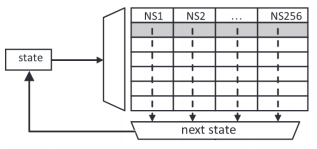
\includegraphics[width=0.4\textwidth]{../src/resources/table.png}}
            \caption{Transition table representation}
            \label{table}
        \end{figure}

        Untuk mengurangi kebutuhan terhadap penanda status akhir, nomor status akan disusun ulang. Status akhir akan diletakkan pada status pertama hingga ke-N. Sedangkan status lainnya termasuk status awal dimulai dari N+1. Dengan demikian, kebutuhan memori untuk penanda akan berkurang. Selain itu, operasi pengecekan dalam kode \emph{kernel} lebih sederhana dan ringan.

    \subsection{Alokasi \emph{Thread}}
        Meskipun \emph{thread} dibangkitkan sangat banyak, banyak juga diantara \emph{thread} yang akan berhenti sangat awal. Sehingga, muatan pencocokan tiap \emph{thread} dapat timpang cukup jauh dan utilisasi GPU rata-rata menjadi rendah. Untuk menunjang utilisasi GPU, \cite{lin2013} mengusulkan alokasi memori yang berulang.

        Dalam satu blok, satu atau beberapa \emph{byte stream} akan ditempatkan sebagai lokasi awal satu \emph{thread}. Misal, dalam blok berisi 4.096 \emph{byte} dengan 512 \emph{thread}, \emph{thread} pertama akan memulai pencocokan pada posisi kelipatan 512. Akibat dari penugasan yang berulang, secara statistik kemungkinan ketimpangan muatan dari masing-masing \emph{thread} akan berkurang \cite{lin2013}. 

    \subsection{Optimasi pada Memori GPU}
        Untuk memaksimalkan utilisasi GPU dan mengurangi latensi akibat transfer data, beberapa metode dapat diterapkan. Salah satu metode yang sangat umum adalah penggunaan \emph{shared memory}. \emph{Shared memory} memiliki latensi yang lebih kecil beberapa kali lipat dibandingkan \emph{global memory}. Namun, ukuran \emph{shared memory} sangat terbatas. Selain itu, \emph{shared memory} harus di-"replikasi" ke setiap \emph{block}. 

        Dengan memanfaatkan sifat \emph{early terminate} pada PFAC, penggunaan \emph{shared memory} dapat dihemat. Transisi dari \emph{state} awal akan selalu diakses namun kemungkinan pencocokan berhenti sangat tinggi \cite{lin2013}. Sehingga transisi ini akan dimuat ke \emph{shared memory} untuk menurunkan latensi ketika pembacaan tabel transisi.

        % kemudian masukan

        Sisa tabel transisi yang masih ada di \emph{global memory} akan ditingkatkan dengan \emph{texture memory}. Diantara keuntungan \emph{texture memory} adalah memiliki \emph{cache} yang lebih besar dan mampu melakukan transpolasi sehingga dapat memanfaatkan \emph{cache} untuk pola yang susah ditebak \cite{lin2013}. Kelemahan \emph{texture memory} data ditulis hanya dari host, cocok dengan skema pencocokan yang melakukan kompilasi kamus sekali dalam satu \emph{rule group}.

        Metode lainnya yaitu dengan melakukan batching dan menyimpan batch dalam pinned memory. Pinned memory adalah memori yang dialokasi di host dan tidak dapat diswap ke disk. Penggunaan pinned memory untuk buffer input dapat menurunkan kemungkinan swappiness untuk ukuran buffer yang besar. Selain itu, pinned memory juga memungkinkan adanya DMA dari host ke device maupun sebaliknya \cite{gnort2008}.

        % Thread reduce bank conflict

\section{Implementation pada Snort}
    \subsection{\emph{Interface} MPSE}
        Dalam mengimplementasi modul pencocokan string, akan digunakan \emph{interface} MPSE (\emph{multi pattern search engine}). Modul deteksi pada Snort akan memuat semua kelas yang mengimplementasi \emph{interface} MPSE. Pilihan metode pencocokan akan diberikan dari konfigurasi sesuai definisi pada file header.

        \emph{Interface} MPSE sendiri berisi beberapa fungsi yang digunakan untuk analisis sebagaimana pada tabel 
        % What provided? And how you implement those interface?

    \subsection{Modules}
        % Connect interface to your design 

\section{Pengujian}
    \subsection{Strategi Pengujian}
        Pengujian dilakukan untuk mendapatkan perbandingan kinerja antara modul yang dikembangkan dan modul yang ada dalam NIDS Snort. Pengujian dibatasi dengan menggunakan konfigurasi \emph{data acquisition} PCAP dengan masukan \emph{file} tcpdump saja. Berkas didapatkan dari arsip DEFCON tahun 2017. \emph{Live testing} tidak diujikan dalam Tugas Akhir ini mengingat kapasitas \emph{network interface} dapat menjadi \emph{bottleneck} sehingga hasil perbandingan tidak akurat.

        Pengujian dilakukan pada komputer dengan spesifikasi seperti pada Tabel ~\ref{test-spec} berikut.
        
        \begin{table}[htbp]
            \caption {Spesifikasi Lingkungan Pengujian}
            \begin{center}
            \begin{tabular}{|l|l|}

\hline
\rowcolor{gray!15}
Komponen & Spesifikasi \\
\hline

Sistem Operasi & Ubuntu 16.04.5 amd64 \\
\hline

CPU & Intel Core i7-7500U CPU @ 2.70GHz × 4 \\
\hline

\emph{Host} RAM & 16 GB \\
\hline

Media Penyimpanan & SSD SATA III 6 Gbps \\
\hline

GPU & NVIDIA GeForce 940MX \\
\hline

Arsitektur GPU & Maxwell \\
\hline

\emph{Compute Capability} & 5.0 \\
\hline

\emph{Dedicated Video} RAM & 2 GB \\
\hline

CUDA \emph{Runtime} & CUDA 8.0 r2 \\
\hline

C/C++ \emph{Compiler} & GCC 5.4.0 \\
\hline

\end{tabular}

            \label{test-spec}
            \end{center}
        \end{table}

        Ada 5 skenario yang akan diujikan dalam penelitian ini: 
        \begin{enumerate}
        
            \item \emph{Baseline} (Aho-Corasick dengan \emph{multithreading} CPU) \\
            \emph{Baseline} akan menggunakan konfigurasi default Snort. Ini menjadi dasar pengukuran kinerja dan kebenaran program yang diimplementasikan pada GPU.

            \item Skenario 1 (PFAC dengan \emph{global memory}) \\
            Skenario ini adalah skenario paling dasar. Optimasi hanya dilakukan pada algoritma tanpa melibatkan optimasi pada latensi GPU.

            \item Skenario 2 (PFAC dengan \emph{shared memory}) \\
            Skenario ini memanfaatkan \emph{shared memory} untuk mengurangi akses ke \emph{global memory}. Transisi \emph{state} awal ke tiap huruf serta \emph{stream} masukan ditampung dalam \emph{shared memory}.

            \item Skenario 3 (PFAC dengan \emph{shared memory} dan \emph{pinned memory}) \\
            Skenario ini mirip dengan skenario 2 dengan tambahan \emph{pinned memory} pada \emph{buffer}. Mekanisme ini diharapkan dapat mengurangi \emph{swappiness} dan memungkinkan DMA (\emph{direct memory access}).

            \item Skenario 4 (PFAC dengan \emph{shared memory}, \emph{pinned memory}, dan \emph{texture memory}) \\
            Skenario ini mirip dengan skenario 3 dengan tambahan \emph{texture memory} pada kamus. Dengan \emph{cache} yang lebih besar, penggunaan \emph{texture memory} diharapkan mengurangi transfer memori.

        \end{enumerate}
        
    \subsection{Pengujian Kinerja}
        asd

\section{Kesimpulan}

% \section{Acknowledgment}

\bibliography{references}
\bibliographystyle{IEEEtran}

\end{document}
